%% ----------------------------------------------------------------
\chapter{Background Research}
%% ----------------------------------------------------------------

\section{Custom Image Compression (jc)}
\label{Custom_comp_research}

Before starting research into image compression standards such as jpeg, a range of general image compression techniques were researched and a selection of these were also implemented in MATLAB, see appendix \ref{chap:Matlab_code}.

\subsection{Overview of Available Methods (jc)}

The idea of image compression is to reduce the amount of data used to describe the image, whilst retaining as much as possible of the information contained in the image. there are two main types of image compression: lossless and lossy.

Lossless compression techniques retain all the information in the image but reduce the size of the data required to describe it, although they can't achieve the same level of compression as lossy techniques. This is usually done by looking for patterns in the data and using these patterns to encode the data in a more efficient way. Some examples of lossless techniques are: run-length encoding or entropy encoding (such as huffman encoding, see section \ref{sec:mikes_huff}). \cite{image_compression}

Lossy compression techniques discard some of the information in the image in order to be able to compress it further than is possible with lossless compression. The two main types of lossy image compression are those based on reducing the information in the colour space (often utilising the way the human eyes works in order to maintain perceived image quality) and those based on transforming the image, usually into a version of the frequency space. \cite{image_compression}

If the image is being compressed so that it can be sent over a medium then this can be done either as a single action: the image is compressed and sent once and any information that is lost is lost forever, or progressively: the image is compressed first with a high loss of information and then the additional information is sent so that the loss of the image being sent reduces as more data is received.

Reducing the resolution of an image could also be considered as lossy compression as it is a very simple method of reducing the amount of data required to describe an image by reducing the information in the image.

\subsection{Downsampling (jc)}
\label{downsampling}

The most obvious method for sending an image progressively is to simply send pixels in such an order that at any time they form a down sampled (lower resolution) version of the image. This way rather than having the image fill in from the top left hand corner the image can become less pixelated as more data is downloaded.

%[] diagram showing how this could work []

%Figure [] ref to above [] show one method that could be used to reconstruct the image progressively.

\subsection{Mike's huffman shizz (mh)} %working title :P
\label{sec:mikes_huff}

\subsection{Mitch's colour space and croma subsampling shizz (ms)} %also a working title
\label{sec:mitch_colour}

\subsection{Transform Based Compression (jc)}
\label{transfom_based}

Some simple progressive encoding was done as an investigation into using the fast fourier transform (FFT) and the discrete cosine transform (DCT) for image compression and how these could be sent progressively.

The fourier transform works by approximating a signal with the sum of sinusoids of different frequencies. The transform function (given an array as an input) outputs an array of complex numbers whose magnitude is the magnitude of the sinusoid at that frequency and whose argument is the phase.

The fast fourier transform (FFT) is an optimised version of the discrete fourier transform (DFT) which implements the fourier transform in discrete rather than continuous space, this enables its implementation by computers.

\begin{equation}
X(k) = \sum_{j=1}^N x(j)\omega _N ^{(j-1)(k-1)}
\label{FFT1_eq}
\end{equation}

where
$ \omega _N = e^{(-2 \pi i)/N} $ is an $N$th root of unity.

Equation \ref{FFT1_eq} is the equation for the 1 dimensional FFT, to implement the FFT in 2 dimensions (as you would need to for an image) you simply take the 1 dimensional FFT of each column and then of each row of the result.

The DCT approximates a signal with the sum of cosine functions of different frequencies. The DCT is similar to the FFT in that it transforms into a frequency space, but the DCT produces strictly real values.

\begin{equation}
F_{u,v} = \alpha(x) \alpha(y) \sum_{x=0}^{M-1} \sum_{y=0}^{N-1} f_{x,y} \cos\Big[\dfrac{\pi}{M}(u+\dfrac{1}{2})x\Big]\cos\Big[\dfrac{\pi}{N}(v+\dfrac{1}{2})y\Big]
\label{DCT2_eq}
\end{equation}

for $0 \leq u \leq M - 1 $ and $0 \leq v \leq N - 1 $

$x$ is the pixel row

$y$ is the pixel column

$u$ is the horizontal DCT frequency

$v$ is the vertical DCT frequency

$
  \alpha(x) = \left\{
  \begin{array}{l l}
    1/ \sqrt{M} & \quad \text{, $u = 0$}\\
    2/ \sqrt{M} & \quad \text{, $1 \leq u \leq M - 1$}\\
  \end{array} \right.
$

$
  \alpha(y) = \left\{
  \begin{array}{l l}
    1/ \sqrt{N} & \quad \text{,$ v = 0$}\\
    2/ \sqrt{N} & \quad \text{, $1 \leq v \leq N - 1$}\\
  \end{array} \right.
$

The 2 dimensional DCT equation is given in equation \ref{DCT2_eq}, this is the equation exactly as implemented in the MATLAB function "dct2" used in [] ref to matlab code in appendix [].

\subsubsection{Whole Image (jc)}

The first algorithm in appendix \ref{chap:Matlab_code} was a progressive scheme based on taking an FFT of the whole image and then reconstructing the image using more and more of the frequency content of the image starting with the lowest frequencies.

\begin{figure}[H]
  \centering
  \begin{tabular}{c c c}
  \subfigure[Image with only low frequency content]{\label{fig:whole_fft_lfc}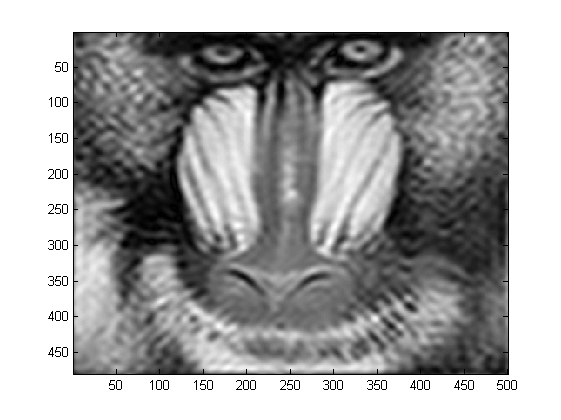
\includegraphics[width=0.3\textwidth]{figures/whole_fft_lfc.png}}&                
  \subfigure[Image with medium and low frequency content]{\label{fig:whole_fft_mfc}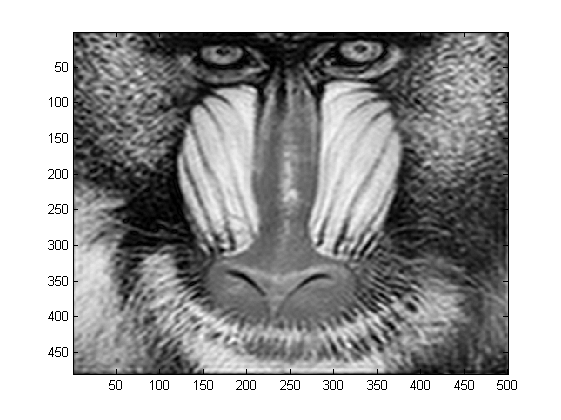
\includegraphics[width=0.3\textwidth]{figures/whole_fft_mfc.png}}&
  \subfigure[Image with all its frequency content]{\label{fig:whole_fft_all}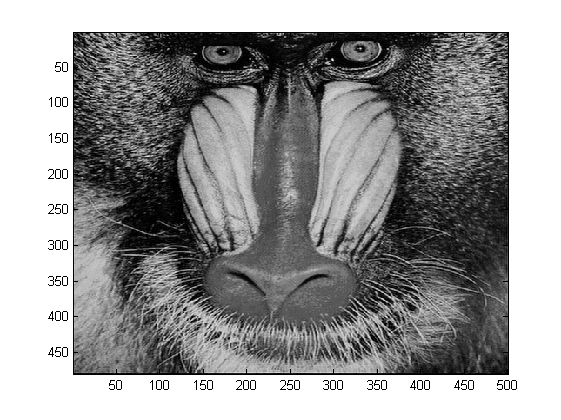
\includegraphics[width=0.3\textwidth]{figures/whole_fft_all.png}}
  \end{tabular}
  \captionof{figure}{Images reconstructed from increasing amounts of an fft of the whole image, see appendix \ref{chap:Matlab_code}}
  \label{fig:whole_fft}
\end{figure}

Figure \ref{fig:whole_fft} how the level of detail in the picture increases as more of the frequency content is used to display it. Potentially the image data could be transmitted so that the low frequency data is received first and additional frequency content is then sent progressively so that the image gains detail smoothly.

The second algorithm in  appendix \ref{chap:Matlab_code} used the DCT rather than the FFT. The advantage of the DCT over the FFT for this purpose is that the FFT generates complex values thereby effectively doubling the amount of data whereas the the DCT only produces real values.

\begin{figure}[H]
  \centering
  \begin{tabular}{c c c}
  \subfigure[Image with only low frequency content]{\label{fig:whole_dct_lfc}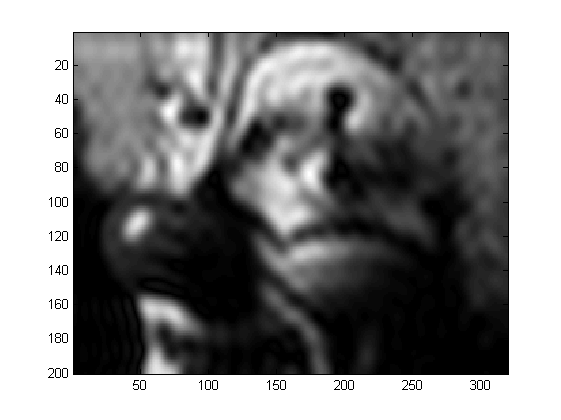
\includegraphics[width=0.3\textwidth]{figures/whole_dct_lfc.png}}&                
  \subfigure[Image with medium and low frequency content]{\label{fig:whole_dct_mfc}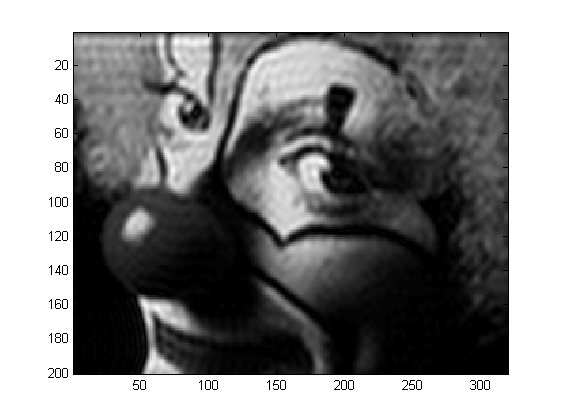
\includegraphics[width=0.3\textwidth]{figures/whole_dct_mfc.png}}&
  \subfigure[Image with all its frequency content]{\label{fig:whole_dct_all}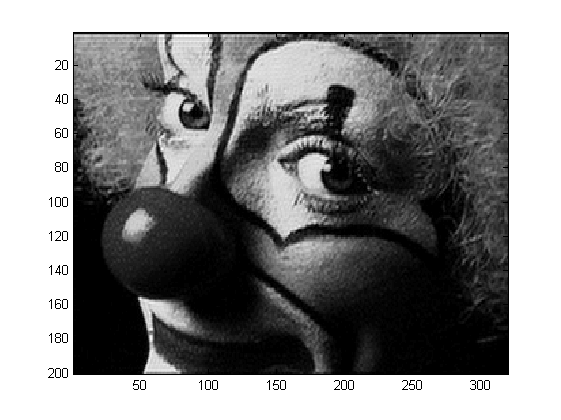
\includegraphics[width=0.3\textwidth]{figures/whole_dct_all.png}}
  \end{tabular}
  \captionof{figure}{Images reconstructed from increasing amounts of a dct of the whole image, see appendix \ref{chap:Matlab_code}]}
  \label{fig:whole_dct}
\end{figure}

\subsubsection{Sectioned Image (jc)}

As FFTs or DCTs can be quite computationally intensive when done with large arrays of values it is sometimes sensible to first break the image down into smaller blocks and then do the transformation on these. This would reduce the complexity of the computations while retaining the same functionality.

\begin{figure}[H]
  \centering
  \begin{tabular}{c c c}
  \subfigure[Sectioned image with only low frequency content]{\label{fig:sectioned_fft_lfc}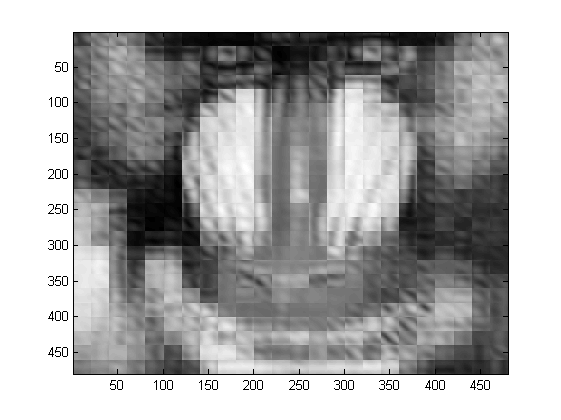
\includegraphics[width=0.3\textwidth]{figures/sectioned_fft_lfc.png}}&                
  \subfigure[Sectioned image with medium and low frequency content]{\label{fig:sectioned_fft_mfc}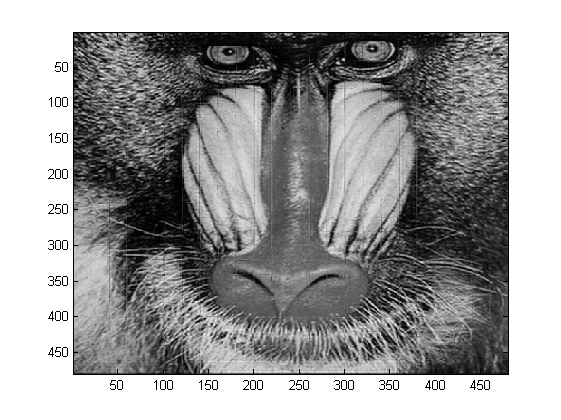
\includegraphics[width=0.3\textwidth]{figures/sectioned_fft_mfc.png}}&
  \subfigure[Sectioned image with all its frequency content]{\label{fig:sectioned_fft_all}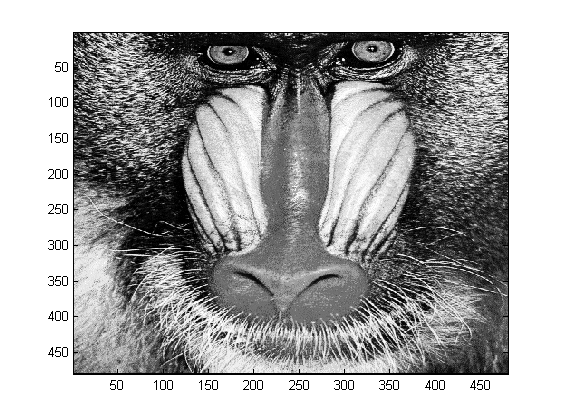
\includegraphics[width=0.3\textwidth]{figures/sectioned_fft_all.png}}
  \end{tabular}
  \captionof{figure}{Images reconstructed from increasing amounts of a fft of sections of the image, see appendix \ref{chap:Matlab_code}}
  \label{fig:sectioned_fft}
\end{figure}

Figure \ref{fig:sectioned_fft} shows much the same as figure \ref{fig:whole_fft} but with the image first broken down into small (definable in the code (see  appendix \ref{chap:Matlab_code}]), 20x20 blocks were used for these images) sections and then the frequency components of these transmitted progressively so that the detail within each section increases as more data is sent and thus the detail of the whole image also increases.

\section{JPEG Image Compression}
The images obtained from the camera will be in the JPEG image format. If the image data is sent to the ground station progressively, it must be necessary to understand how a JPEG image is structured to reconstruct the encoded image. Unlike raw image data, which can easily be read continuously, JPEG files have already been compressed and contain information which must first be read to properly decompress the image.

\subsection{JPEG structure}
A JPEG file can be separated into two main parts. The first part of the JPEG file is composed of segments containing information concerning various properties of the image which must be read in order to recover the image from its compressed form. The second part contains the entropy-encoded image data, which can be decoded using the information provided from the headers of the file.  

The segments which make up the image file properties are indicated by header markers. ``Each marker is immediately preceded by an all 1 byte (0xff).'' (Header guide) This marker is then followed by a marker identifier byte specific to that segment type. The 0xff value will always indicates the start of the header in this part, but is treated differently in the image data stream. ``If a 0xff byte occurs in the compressed image data either a zero byte (0x00) or a marker identifier follows it.'' (Header guide) 0xff bytes followed by a zero byte are read in as the hexadecimal value 0xff and the 0x00 byte is ignored entirely. 0xff bytes not following this a 0x00 byte are considered to be the header byte of the next segment. If the segment contains useful information before the next marker identifier, it is then followed by two bytes specifying the total length of the segment (in bytes). For the SOS segment, this does not include the entropy-encoded image data.

\subsubsection{JPEG Segments}
The number of headers found within a JPEG image file is not constant between images. The JPEG headers are capable of storing most of the metadata related to an image, not all of which is necessary for the decompression of the image. The following headers are those which contain all the information necessary for a successful decompression of the JPEG image, as well as those which can be found in all JPEG images. The number in brackets next to the segment name is the unique marker identifier value which appears directly after the 0xff marker indicator byte. All numerical values obtained from the byte stream are unsigned. ``DQT, DHT, DRI and SOF may line up in any order, but must be recorded after APP1 (or APP2 if any) and before SOS.'' (Exif)

\paragraph*{SOI: Start Of Image (0xd8)}
This header identifies the start of the image and can be found in all JPEG images. This is the first header to be read in a JPEG file. This header does not contain any information to be stored by the decompression algorithm, but can be useful for differenciating multiple JPEG images from a single data stream.

\paragraph*{APP0: JFIF application segment (0xe0)}
There can be many APP segments in a single image. Subsequent APP segments are named ``APP\emph{n}'' with a marker identifier of 0xe\emph{n} with \emph{n} being the number of the APP segment. This segment does not contain any information necessary to the decompression algorithm used, so all APP segments ignored.

\paragraph*{SOF0: Start Of Frame (0xc0)}
``SOF is a marker code indicating the start of a frame segment and giving various parameters for that frame'' (Header guide) /this indicates that the image is a ``DCT-based JPEG, and specifies the width, height, number of components, and component subsampling (e.g., 4:2:0)'' as well as the data precision (in bits/sample) of an image. (narcap) From the component subsampling information, the size of the Minimum Coded Unit (MCU) which make up the JPEG image. Just like the APP segments, there can be multiple start of frame segments in more complex images, but the images sent by the camera will only need the information contained in the first SOF segment.

\paragraph*{DHT: Define Huffman Table(s) (0xc4)}
This segment defines the properties of one or many Huffman table(s) (HT) which will be used to decode the entropy-encoded image data. ``A single DHT segment may contain multiple HTs, each with its own information byte.'' This segment includes the number of the HT as identified by the image data and the type of the HT (either DC or AC) It also stores the ''number of symbols with codes of length 1..16, the sum (n) of these bytes is the total number of codes, which must be $\leq$ 256'' as well as ``the symbols in order of increasing code length ( n = total number of codes )'' (Header guide). In practice, a single image can also contain multiple DHT segments which all share the same marker identifier. 

\paragraph*{DQT: Define Quantization Table(s) (0xdb)}
This segment defines the properties of one or many quantization table(s).

\paragraph*{SOS: Start Of Scan (0xda)}
This segment gives various scan-related parameters and is the last segment preceding the entropy-encoded image data. This segment associates each component in the scan with the appropriate AC and DC Huffman table by their ID number. 3 ignorable bytes seperate this segment from the image data. 

\paragraph*{EOI: End Of Image (0xd9)}
This header identifies the end of the image. ''It is possible that the end of the image is reached without finding the EOI marker. In this case, the image is technically malformed but the situation is tolerated and handled as if the EOI marker was found.`` (winzip) 

\subsubsection{Entropy-encoded image data}
(Exif)

\subsection{JPEG Header Information Extractor}

\subsection{Progressive Display of Image}

\section{Existing Hardware and Software}
Research concerning the payload and the associated software goes here...

\section{SkyCircuits Autopilot}

%\section{Hardware Selection}
%Research justifying hardware choice goes here...

